
\documentclass [PhD] {uclathes}

% \input {mymacros}                         % personal LaTeX macros
\usepackage[round]{natbib}
\def\newblock{\ }
\usepackage[T1]{fontenc}
\usepackage{times}
\usepackage{latexsym}
\usepackage[utf8]{inputenc}
\usepackage{graphicx}
\usepackage{multirow}
\usepackage{microtype}
\usepackage{inconsolata}
\usepackage{subcaption}
\usepackage{amsfonts,amssymb}
\usepackage{booktabs}


%%%%%%%%%%%%%%%%%%%%%%%%%%%%%%%%%%%%%%%%%%%%%%%%%%%%%%%%%%%%%%%%%%%%%%
%
% Usually things live in separate flies.
%
% \input {prelim}                           % preliminary page info

%%%%%%%%%%%%%%%%%%%%%%%%%%%%%%%%%%%%%%%%%%%%%%%%%%%%%%%%%%%%%%%%%%%%%%%%
%                                                                      %
%                          PRELIMINARY PAGES                           %
%                                                                      %
%%%%%%%%%%%%%%%%%%%%%%%%%%%%%%%%%%%%%%%%%%%%%%%%%%%%%%%%%%%%%%%%%%%%%%%%

\title          {Mitigating Gender and Racial Bias \\
                in Automated English Speaking Assessment}
\author         {Alexander Kwako}
\department     {Education}
% Note:  degreeyear should be optional, but as of  5-Feb-96
% it seems required or you get a year of ``2''.   -johnh
\degreeyear     {2023}

%%%%%%%%%%%%%%%%%%%%%%%%%%%%%%%%%%%%%%%%%%%%%%%%%%%%%%%%%%%%%%%%%%%%%%%%

\chair          {Michael H. Seltzer}
\member         {Mark P. Hansen}
\member         {Li\ Cai}
\member         {Kai-Wei\ Chang}

%%%%%%%%%%%%%%%%%%%%%%%%%%%%%%%%%%%%%%%%%%%%%%%%%%%%%%%%%%%%%%%%%%%%%%%%

\dedication     {\textsl{To my partner, Kathryn, and my mom, Jamie, \\
                                  who deserve credit for at least 95\% of all my good fortune, \\
						  including having finished this dissertation, \\
						  and having been able to study with the incredible faculty at UCLA}}

%%%%%%%%%%%%%%%%%%%%%%%%%%%%%%%%%%%%%%%%%%%%%%%%%%%%%%%%%%%%%%%%%%%%%%%%

\acknowledgments {
I would like to express my deepest gratitude and appreciation to all those who have contributed to the completion of this dissertation. I extend my heartfelt thanks to my advisor, Mike Seltzer, for accepting me into the Social Research Methodology division, and for providing endless support, reassurance, and encouragement to follow my interests. And whose great taste in music has given me the chance to hear new jazz and rock music and musicians! I am truly grateful for his mentorship and constant encouragement throughout this journey.

My thanks go out to all the members of my dissertation committee. To Mark Hansen, for encouraging me to apply for the Transdisciplinary Research Acceleration Grant, for his belief in and guidance throughout this project, and for providing thoughtful and insightful feedback at every step of the way. To Li Cai, for always being available for a statistical consult, and for sharing the breadth of his expertise and wisdom about language assessment. To Kai-Wei Chang, for his commitment to sharing his knowledge of Natural Language Processing with others outside of the Computer Science department, for embarking on this interdisciplinary project, and for generously sharing his resources with us in Education. 

I would also like to extend my appreciation to John Rogers, for being a role model of great leadership looks like, and for showing me how scholarship can make an impact in the world. And thanks to Bill Sandoval, who introduced me to educational research, and who welcomed me on his team in my most formative years at UCLA. 

My deepest gratitude goes out to my family and my partner. To my mom, for her commitment to my education, for her unconditional love and support, and for cultivating my intellectual curiosity and openness to new ideas. To my dad, for his calm support, and his veneration for serious thinking. To my brother, for teaching me the power of tenacity, and for being a vigilant friend inside science and math and beyond. And of course to my partner, Kathryn, to whom I owe my present happiness, who taught me that I could love writing and thinking as an academic, whose curiosity and ways of thinking are an endless source of inspiration. 

To all those who have supported me that I have failed to mention, I offer my sincere appreciation. Your contributions, both big and small, have played a significant role in the completion of this dissertation. Thank you for being a part of this transformative experience. 
}



%%%%%%%%%%%%%%%%%%%%%%%%%%%%%%%%%%%%%%%%%%%%%%%%%%%%%%%%%%%%%%%%%%%%%%%%

\vitaitem   {2010}
                {B.A.~(Liberal Arts),
                St. John's College.}
\vitaitem   {2017}
                {M.A.~(Education), 
		UCLA.}
\vitaitem   {2016--2018}
                {Graduate Student Researcher, Developing Teachers' Capacity to Promote Argumentation in Secondary Science, UCLA.
                Collaborated with secondary school science teachers on implementing Next Generation Science Standards, with a focus on classroom discussion.}
\vitaitem   {2018--2022}
                {Graduate Student Researcher, Institute for Democracy, Education, and Access, UCLA.
                Analyzed national survey of U.S. public high school principals. 
		Prepared public-facing reports and articles for academic journals.}
\vitaitem   {2021--2022}
                {Graduate Student Researcher, Center for Research on Evaluation, Standards, and Student Testing, UCLA. 
		Contributed to university efforts to understand effects of COVID on undergraduate experience. 
		Refined survey to understand state-level approaches to English Language Learner pedagogy.}
\vitaitem   {2021--2022}
                {Researcher, Transdisciplinary Research Acceleration Grant, UCLA.
		Developed proposal to study the use of debiasing techniques in automated English speaking assesment.}
\vitaitem   {2022--2023}
                {Dissertation Year Fellowship, UCLA.
		Continued study of measurement and mitigation of bias in automated English speaking assessment.}

%%%%%%%%%%%%%%%%%%%%%%%%%%%%%%%%%%%%%%%%%%%%%%%%%%%%%%%%%%%%%%%%%%%%%%%%

\publication    {\textsl{Patterns of classroom talk through participation in discourse-focused teacher professional development.}
	                Proceedings of the 13th Annual International Conference of the Learning Sciences, 2018}
\publication    {\textsl{What is this thing called a mechanism? Findings from a review of realist evaluations.}
                	New Directions for Evaluation, 2020.}
\publication    {\textsl{Do Adolescents Want More Autonomy? Testing Gender Differences in Autonomy Across STEM.}
	                Journal of Adolescence, 2021.}
\publication    {\textsl{Do Politics in Our Democracy Prevent Schooling for Our Democracy? Civic Education in Highly Partisan Times.}
	                Democracy \& Education, 2021.}
\publication    {\textsl{Using Item Response Theory to Measure Gender and Racial Bias of a BERT-based Automated English Speech Assessment System.}
                	Proceedings of the 17th Workshop on Innovative Use of NLP for Building Educational Applications, 2022.}
\publication    {\textsl{Principals’ Responses to Student Gun Violence Protests: Deter, Manage, or Educate for Democracy.}
                	Teacher’s College Record, 2023.}

%%%%%%%%%%%%%%%%%%%%%%%%%%%%%%%%%%%%%%%%%%%%%%%%%%%%%%%%%%%%%%%%%%%%%%%%

\abstract{
Automated assessment using Natural Language Processing (NLP) has the potential to make English speaking assessments more reliable, authentic, and accessible. Yet without careful examination, NLP may exacerbate social prejudices based on gender or native language (L1). Current NLP-based assessments are prone to such biases, yet research and documentation are scarce. Considering the high stakes nature of English speaking assessment, it is imperative that tests are fair for all examinees, regardless of gender or L1 background. This project addresses the need for studies in English speaking assessment through a series of three studies. In Study 1, I measure the accuracy of automated transcription, a key component of automated speaking assessments. In Study 2, I analyze a specific type of bias known as differential item functioning (DIF), and determine what patterns of DIF are present in human rater scores; moreover, I evaluate whether patterns of DIF are exacerbated by a pretrained, large language model (LLM) known as BERT. Lastly, in Study 3, I compare two approaches of mitigating DIF. Results from Study 1 indicate that there are indeed biases in automated transcription, however these do not translate into higher or lower scores. In Study 2, it is shown that BERT does (albeit to a small degree) exacerbate human rater biases. Finally, Study 3 demonstrates that it is possible to debias human and automated scores; however, the two approaches have serious limitations, particularly when the source of DIF is unknown. 
}

%%%%%%%%%%%%%%%%%%%%%%%%%%%%%%%%%%%%%%%%%%%%%%%%%%%%%%%%%%%%%%%%%%%%%%%%



\begin {document}
\makeintropages

%%%%%%%%%%%%%%%%%%%%%%%%%%%%%%%%%%%%%%%%%%%%%%%%%%%%%%%%%%%%%%%%%%%%%%
%
% Ordinarily each chapter (at least) is in a separate file.
%
%\input {chapter1}                         % Chapter 1 of dissertation
%\input {chapter2}                         % Chapter 2
%\input {chapter3}                         % etc.
%\input {chapter4}
%\input {chapter5}
%\input {chapter6}
%\input {chapter7}
%\input {chapter8}

\chapter{Introduction}

Automated assessment of non-native (L2) English speaking proficiency is made possible by recent advances in Natural Language Processing (NLP). Researchers have shown, for instance, that pretrained large language models (LLMs) can accurately replicate human rater scores in English speaking assessment \citep{wang2021automated}. Although applications of NLP present new opportunities for language assessment, recent studies have revealed that NLP can propagate and, in some cases, amplify negative stereotypes of marginalized groups \citep{blodgett2020}. Societal biases become embedded in NLP models, which may lead to unfair scoring, e.g., where examinees of a particular racial background are systematically given lower scores than others (Wang et al., 2018). Perhaps more commonly, biases of NLP-based assessments are not examined at all \citep[e.g.][]{collier2020test, ormerod2022automated}). 

Considering how widespread and high stakes English speaking assessments are at both the primary and secondary education levels \cite{cimpian2017, ets2005}, it is imperative that these assessments be fair for all students, regardless of gender or racial background. This dissertation presents a set of three studies aimed to address the need for deeper analyses of bias in automated assessment of non-native (L2) English speaking. 

This study draws on data from the English Language Proficiency Assessment for the Twenty-First Century (ELPA21), a collaborative of 7 state education agencies in the U.S. \citep{huang2018english}. Both the quantity and quality of data, as well as the consortium’s openness to research, make ELPA21 an ideal context in which to study biases of automated assessments.

In addition to examining gender and racial biases, I explore the use of debiasing techniques to mitigate such biases \citep{sun2019mitigating}. As debiasing is a relatively new area of research and has not yet been applied to language assessments, the primary goal is to examine advantages as well as disadvantages afforded by various approaches. This project addresses important gaps in English speaking assessment systems, so that NLP may be applied responsibility, in order to ensure fairness for all examinees.

\section{Automated speaking assessments}

English language assessment is mandated in the United States by the Every Student Succeeds Acts \citep{essa2015}. Tests are administered to over 4 million K-12 students annually \citep{irwin2021report} and, for university admissions, over 500,000 students take the Test of English as a Foreign Language \citep[TOEFL][]{ets2005}. Importantly, these test are often high stakes \citep{cimpian2017}.

In order to cut costs and meet the rising demand for English language assessments, some test developers have transitioned to fully automated assessment systems. These systems automate all aspects of English language assessment, including speech and writing, which in the past have been scored solely by human raters \citep{evanini2017approaches}. Several researchers, however, have questioned the fairness of automated speaking assessment systems, particularly for examinees of minority groups \citep{wang2018monitoring, collier2020test}.

\section{Advantages of automation}

While the advantages of NLP-based assessments are typically framed in terms of efficiency and affordability, NLP also has the capacity to improve reliability and even advance social justice-oriented goals. In the testing literature, it is well known that human raters are subject to cognitive and social biases \citep{engelhard2002monitoring}. Psychometricians often categorize these biases based on whether raters tend toward excessively severity or leniency, or whether they are prone to halo effects \citep{saal1980}. These biases persist even in the face of training and monitoring \citep{engelhard1994examining}, indicating that they operate at an unconscious level \citep{spencer2016}, which make them difficult to address.

Automated systems, in contrast to human raters, are not prone to the same kind of inconsistencies or unconscious bias. Indeed, automated scoring can promote fidelity of scores by identifying and mitigating human rater errors \citep{bejar2011validity}. \citet{wang2018monitoring} have demonstrated how automated systems can be used to identify overly lenient or harsh human raters in the TOEFL exam: A similar approach, though not yet attempted, could be used to identify raters with biases against minoritized groups.

While not prone to the same sorts of errors as human raters, automated systems can still be biased. However, there are methods for identifying and mitigating such biases in NLP-based applications. \citet{zhao2018gender}, for example, have shown how it is possible to debias an NLP-based application that resolves coreferences (e.g., identifying subjects of sentences when pronouns are ambiguous). Originally, the application was more likely to ascribe historically male professions (such as politician or doctor) to male subjects; however, after supplementing the corpus with less biased data, the model became more gender-neutral in its coreference resolutions. Whether social biases are present in humans or in automated systems, they can be measured and mitigated with careful planning and engineering.

\section{Bias and debiasing}

There is little research on bias in automated testing of English speaking proficiency. In order to illustrate what sorts of problems might occur with these systems, I consider two hypothetical examples of how biases might become embedded in automated English language assessment systems, and how bias reduction techniques could be used to address them.

\subsection{Insufficient training data for automated speech recognition}

Automated speech recognition (ASR) systems have been shown to be less accurate for non-White speakers (Koenecke et al., 2020) and, in some cases, less accurate for women (Tatman, 2017; Tatman and Kasten, 2017). These disparities may be due to lack of representation in the data itself \citep[e.g.][]{zhao2018gender}. In English language assessment, a less accurate ASR system will generate less accurate transcripts, which equates to less accurate scores for language-minority examinees. Beyond transcription accuracy, when ASR systems are also used to generate linguistic features (e.g., pronunciation scores), language-minority examinees may be given lower scores.

One possible debiasing solution for language assessment systems that lack sufficient data for language-minority groups is to implement a filtering model. The filtering model could flag some responses as non-scorable and send them to human raters for review. Bypassing automated scoring in some cases may help to ensure that certain examinees (e.g., who are known to have less accurate transcripts) are not penalized by the ASR system.

A more comprehensive solution would be to use a technique known as data augmentation \citep[e.g.][]{zhao2018gender}. A simple version of data augmentation is simply to duplicate the data of underrepresented groups to artificially make them more representative. Although requiring more effort, it is also possible to apply various transformations to audio data (e.g., changing the pitch of male and female respondents, or mixing and matching speakers with different accents). These transformations would help to prevent the model from learning construct-irrelevant features like pitch or accent. This approach would remove the ability of the model to learn differences in race or gender at the data-level.

\subsection{Implicit bias in human ratings}

Scholarship on implicit bias demonstrates that human behavior is influenced unconsciously and in diverse contexts by culturally-embedded associations \citep{greenwald2006implicit}. These associations, including negative stereotypes about underrepresented groups, typically operate independently of individuals’ explicit attitudes \citep{karpinski2001attitudes} and they are often activated by peripheral cues \citep{spencer2016}.

In the context of English speaking proficiency, it is possible that examinees’ accents may trigger human raters’ implicit biases. For instance, as a whole, the U.S. population has an implicit bias against faces that have Arabic features \citep{park2007implicit}; it is possible that hearing a Middle Eastern accent might prompt a rater from the U.S. to (unwittingly) give a lower score. Based on research on the salience of peripheral cues, such bias would be more likely to be present when raters hear adult voices with heavier accents, and for raters who are distracted, hungry, or otherwise on autopilot.

In addition to filtering and data augmentation, another technique that would ameliorate the propagation of implicit bias is retraining the model using adversarial neural networks. Widely applicable to a number of problems encountered in deep learning, adversarial networks actively prevent the model from learning certain information. Following the example of \citet{zhang2018mitigating}, it would be possible to ensure that the language model is unable to predict the ethnic origin of examinees’ responses. In removing its ability to infer race or gender, it may also remove the source of implicit bias.

\section{Overview of study design}

The general research design involves four main components: using automated transcription services to generate text from speech, constructing a language model to score examinees’ (transcribed) text, measuring gender and racial bias via analysis of differential item functioning (DIF), and exploring solutions for debiasing models. Speaking items were selected from the English Language Proficiency Assessment for the 21st Century (ELPA21), to reflect a range of ages and expected duration of response. It is hypothesized that adult voices and longer items will trigger more implicit bias, and hence will be more likely to show DIF. As a part of this analysis, I also examine biases in the automated speech recognition (ASR) system by calculating word error rate (WER) of speech-to-text transcripts. 

In this study of racial and gender bias, I focus on a specific type of bias known as differential item functioning (DIF), common in educational and psychological assessment \citep{aera2014}. Briefly, DIF occurs when equally proficient individuals who belong to different groups (e.g., male and female) are given consistently different (i.e., higher or lower) scores for certain items. Although items in all large-scale assessments have been analyzed for DIF, including ELPA21 \citep{anderson2015elpa21}, there are multiple methods of testing for DIF, and patterns of DIF may change over time (e.g. since the initial development of the test). The specific approach that I use to identify DIF is specifically suited to the context of this research study.

Debiasing NLP-based applications is a relatively new field of research. It will be of interest to compare multiple methods of debiasing, and to determine how well each addresses DIF.

These research goals are organized in three interconnected studies: 

\begin{enumerate}
    \item In Study 1, I quantify the biases of large-scale, automated transcription services, by comparing average WER, disaggregated by gender and L1 background.
    \item In Study 2, I examine DIF in human raters and an LLM-based automated scoring system, to see if the LLM-based automated scoring system introduces or exacerbates any patterns of DIF. 
    \item In the third study, I explore two techniques to mitigate bias in automated systems, each with their own advantages and limitations.
\end{enumerate}

The specific research questions that each study addresses are enumerated in the respective chapters. Since they share a common aim, however, they also draw from the same source of relevant literature and methods, which will be discussed altogether.



\chapter{Literature Review}

This study is situated at the intersection of (1) English speaking assessment, (2) measurement of bias, and (3) language modeling. With respect to English speaking assessment, I review (a) relevant literature on the prevalence and high stakes nature of English speaking assessment in the United States, and (b) automated speaking assessment systems currently in use. With respect to measurement of bias, I discuss (a) the impact of gender and L1 on L2 English speaking proficiency, and (b) differential item functioning (DIF) both in general and as it relates to English speaking assessment. Finally, with respect to language modeling, I review research on large language models (LLMs), how these models become embedded with societal biases, and how some researchers have been able to debias LLMs. 

\section{English speaking assessment}

\subsection{English speaking assessment in the United States}

English language assessment is widespread and often holds high stakes for examinees in the United States. The Every Student Succeeds Acts \citep{essa2015} requires states to administer English language assessments to all students from non-English speaking homes, and tests are administered to over 4 million K-12 students annually \citep{irwin2021report}. English language assessments are also prevalent at the post-secondary level: Every year, over 500,000 examinees take the Test of English as a Foreign Language (TOEFL), administered by Educational Testing Service \citep{ets2005}, and 3.5 million people take the International English Language Testing System \citep{ielts2023}. In terms of real-world impact, many universities require applicants to score above a certain threshold of proficiency on the TOEFL or IELTS as an admission requirement. For K-12 students, being classified as an “English learner” decreases high school graduation rates and college-going behavior \citep{johnson2019effects}.

Nearly all language assessments include speaking as one of four language proficiency domains, along with listening, reading, and writing \citep{ccsso2012framework}. At the K-12 level, speaking tasks are usually open-ended, yet have a narrow contextual focus; for instance, students are asked (via written or verbal prompt) to describe what is happening in a picture \citep{luoma2004assessing}, At the post-secondary level, examinees are given more challenging tasks, e.g., talking about a particular topic for several minutes. For most assessments, examinees speak into a microphone and responses are scored by a human rater or an automated system. Using a slightly different approach, \citet{ielts2023} employees trained interviewers to administer and score speaking proficiency in a face-to-face setting.

For K-12 students, the majority of states administer assessments developed by one of two consortia, World-Class Instructional Design and Assessment (WIDA) or English Language Proficiency Assessment for the 21st Century (ELPA21). Neither consortium currently uses automated speaking assessment: Rather, for speaking items, test-takers speak into a microphone for 5-10 seconds, whereafter their responses passed along to human raters to score.

There are two states, however, that do use automated assessment for K-12 speaking proficiency. Both states use systems developed and administered by Pearson. The Texas English Language Proficiency Assessment System (TELPAS) uses Versant, one of the first automated speaking proficiency assessments, originally developed for large businesses and administered over the telephone \citep{pearson2019versant}. Given the lack of validity studies and potential unreliability of its automated system, TELPAS’ recent switch to Versant has sparked some skepticism among academics \citep{collier2020test}. Pearson also helped to develop the speaking assessment for the Arizona English Language Learner Assessment (AZELLA), seemingly independent of Versant \citep{johnston2019using}. At the post-secondary level, TOEFL uses an automated speaking assessment system known as SpeechRater, developed by researchers at ETS \citep{chen2018automated}.

\subsection{Current NLP-based automated speaking assessments}

\citet{chen2018automated} identify four primary components of automated speaking assessment systems: (1) an automated speech recognition (ASR) system, which includes speech-to-text transcription, (2) the extraction of linguistic features from audio and text data, (3) a filter model to identify non-scorable responses (e.g., those with audio errors or potential plagiary), and (4) a scoring model to combine linguistic features into a single score.

Depending on the purpose or sophistication of the automated assessment system, some of the above steps may be combined or omitted. Pearson, for instance, appears to omit the filter model (step 3) for TELPAS and AZELLA. In a different vein, \citet{chen2018end} have experimented with combining steps 1, 2, and 4 into a single end-to-end model. (Models are described as end-to-end when multiple intermediate processes get subsumed within a single architecture.) Although the performance of end-to-end models can be impressive, they are a black box—that is, the linguistic features that the model learns and uses to score examinees’ responses are hidden. For this reason, it can be challenging to interpret or debug end-to-end models.

\subsubsection{(1) Automated speech recognition}

The ASR system built by ETS is comprised of multiple parts, and used for multiple purposes. Under the hood, it uses a Hidden Markov Model to parse phonemes (i.e. syllables), an n-gram model to track word dependencies, and a weighted finite state transducer to limit the search space \citep{qian2019automatic}. Combined, these three components are able to generate transcripts and assign probabilities to text. The transcripts are used for further data processing, while the probabilities associated with the transcripts may be used as a linguistic feature (referred to as the “Average ASR Confidence Score”) in the scoring model \citep{zhang2019assessing}.

Training ASR systems requires a prolific amount of labeled data (i.e., audio files accompanied by accurate transcripts). The exact amount of training data required to build an ASR system depends on the complexity of the speech. For speech assessment purposes, \citet{qian2019automatic} suggests on the order of a million words; \citet{evanini2017approaches} suggests 200-300 hours of speech. Data can be supplemented with external speech corpora, e.g., the Switchboard corpus \citep{godfrey1997switchboard}, in order to improve the accuracy of speech-to-text transcription; but ensuring recording quality across data sources can be challenging \citep{qian2019automatic}.

Even with external data, there may yet remain a significant amount of transcription error. A common index of transcription accuracy is word error rate (WER), which is the ratio of the total number of errors (i.e. erroneous insertions, deletions, or substitutions) to the total number of words in a given transcript or corpus \citep{qian2019automatic}. (See Section XX for details regarding how WER is computed.) Human-human transcription of non-native speech typically yields a WER of 15-20\% \citep{zechner2009}. SpeechRater comes close to human parity, with a WER of 23\% for non-native spontaneous speech \citep{tao2016exploring}. AZELLA has a higher WER of 35\% \citep{cheng2014automatic}. By contrast, human-human WER of native speech cam be as low as 5\% \citep{xiong2016achieving}.

One of the significant challenges of transcribing non-native speech is faithfully capturing errors. Rather than reproduce errors, ASR systems tend to predict a similar (grammatically correct) phrase. One internal study showed that SpeechRater failed to capture 70\% of non-native speakers’ grammatical errors \citep{yoon2019features}.

\subsubsection{(2) Linguistic features}

Once audio data has been transcribed, linguistically-relevant features are extracted from text and audio data. Linguistic features are typically defined a priori, in alignment with standards of speaking proficiency \citep[e.g.][]{brown2005examination}. For instance, to assess fluency, SpeechRater calculates (among other things) the number of pauses, the duration of pauses, and the number of words per second in examinees’ speech \citep{hsieh2019features}. To assess vocabulary, SpeechRater calculates the number of unique words that examinees use \citep{yoon2019features}. In TOEFL, over 60 linguistic features have been examined as candidates for speech assessment. (Note: In an end-to-end model, these a-priori decisions about which linguistic features to use are not possible, since the features are latent.)

\subsubsection{(3) Filter model}

A filter model helps to reduce error in the automated system by identifying “non-scorable responses” \citep{loukina2019scoring}. Such responses may have had audio issues; alternatively, they may be the result of uncooperative examinees or plagiary. In such cases, examinees’ responses may bypass the automated assessment system, and instead be designated for human rating. Common technical difficulties include the presence of background noise and mechanical issues with recording devices; as described above, ASR systems can be sensitive to slight discrepancies in audio quality, which may produce inaccurate transcripts and, subsequently, inaccurate test scores. There are also instances in which a filter model can be used to identify examinees who are cheating or otherwise gaming the system.

The filter model is helpful in improving the ASR system by acting as a manual override. Automated assessment systems are known to have certain weaknesses, and rather than build a system that is capable of handling every type of exception, it may be more cost-effective to bypass the automated assessment system in certain cases.

\subsubsection{(4) Scoring model}

The scoring model combines linguistic features to produce a summative language proficiency score for examinees \citep{loukina2019scoring}. Finding an appropriate scoring model also requires a lot of data. In order to train a scoring model for complex constructed item types, \citet{zechner2019summary} suggests having at least 10,000-20,000 pre-scored responses. More complicated scoring models, however, might require significantly more data.

TOEFL uses linear regression, wherein features are weighted and selected using a LASSO-based method \citep{loukina2015feature}. The primary rationale for using linear regression is that it is relatively transparent and easy to communicate; \citet{loukina2019scoring} report that ETS has experimented with more complex scoring models, e.g., random forests, but they were not worth the 2-3\% improvement in accuracy. \citet{zechner2019summary} reports that, at the item-level, their scoring model is more reliable than human-human reliability coefficients ($r$ = 0.65, compared to $r$ = 0.55-0.60). In contrast to TOEFL, AZELLA combines features using a deep learning model with a single layer of latent variables \citep{cheng2014automatic}.







\chapter{Methods}

\subsection{Data}

This study draws on data from the English Language Proficiency Assessment for the 21st Century (ELPA21), a consortium involving 7 state education agencies in the U.S. \citep{huang2018english}. To maintain confidentiality, certain details regarding test items and examinees are omitted. 

Analyses focused on two grade-bands (2–3 and 9–12) which corresponded to two tests administered during the 2020–2021 school year. For items in the Speaking domain, examinees spoke into a microphone for up to two minutes, after which their responses were sent to human raters who assigned holistic integer scores based on item-specific scoring rubrics. All verbal responses in ELPA21 are currently scored by human raters Raters are trained and monitored over time to ensure consistency \citep{engelhard2002monitoring}. 

\subsection{Sample design and demographics}

The sampling frame included all examinees in grade-bands in 2–3 or 9–12 who met the following inclusion criteria: answered all three speaking items included in this study; answered enough items in each of the other three domains to receive domain-specific scores; and had gender and L1 demographic information available. Furthermore, to limit the scope of the study, we excluded examinees who had an IEP or 504 Plan, examinees with non-binary gender, and examinees whose L1 was other than one of the ten L1s analyzed in this study. 

From the sampling frame, we sampled 15,000 students.\footnote{The size of our sample was limited, in part, by the cost of automated transcription.} We included all examinees whose L1 was one of the nine L1 focal groups (Table \ref{smp_dscr}). The remainder of examinees were randomly sampled from Spanish speakers. 

\begin{table*}[htbp]
\centering
% \small  % comment out this line if wanted bigger font size
\begin{tabular}{lccccccc}
\toprule
    & \multicolumn{3}{c}{\textbf{Grade Band 2-3}} & \multicolumn{1}{c}{ } & \multicolumn{3}{c}{\textbf{Grade Band 9-12}} \\
    \cline{2-4}
    \cline{6-8}
     & \textbf{n} & \textbf{\%} & \textbf{Avg. Proficiency} & & \textbf{n} & \textbf{\%} & \textbf{Avg. Proficiency} \\
    \midrule
    \textbf{All} & 8377 & 100 & 0.18 (0.91) & & 6623 & 100 & 0.16 (0.93) \\
    \textbf{Gender} &  &  &  & &  &  &  \\
    \hspace{3mm} Male & 4310 & 51.5 & 0.13 (0.9) & & 3648 & 55.1 & 0.14 (0.94) \\
    \hspace{3mm} Female & 4067 & 48.5 & 0.23 (0.92) & & 2975 & 44.9 & 0.2 (0.92) \\
    \textbf{L1} &  &  &  & &  &  &  \\
    \hspace{3mm} Spanish & 4205 & 50.2 & 0.08 (0.85) & & 3481 & 52.6 & 0.23 (0.92) \\
    \hspace{3mm} Marshallese & 692 & 8.3 & -0.0 (0.86) & & 891 & 13.5 & -0.05 (0.75) \\
    \hspace{3mm} Russian & 862 & 10.3 & 0.28 (0.9) & & 375 & 5.7 & 0.49 (0.86) \\
    \hspace{3mm} Vietnamese & 522 & 6.2 & 0.41 (0.9) & & 402 & 6.1 & 0.36 (0.93) \\
    \hspace{3mm} Arabic & 499 & 6 & 0.33 (0.88) & & 414 & 6.3 & 0.06 (0.86) \\
    \hspace{3mm} Mandarin & 439 & 5.2 & 0.88 (0.89) & & 203 & 3.1 & 0.44 (1.02) \\
    \hspace{3mm} Hindi & 416 & 5 & 0.75 (0.82) & & 185 & 2.8 & 0.67 (0.82) \\
    \hspace{3mm} Mayan & 238 & 2.8 & -0.66 (0.88) & & 258 & 3.9 & -0.84 (0.95) \\
    \hspace{3mm} Persian & 295 & 3.5 & -0.05 (1.01) & & 197 & 3 & -0.07 (0.94) \\
    \hspace{3mm} Swahili & 209 & 2.5 & 0.22 (0.87) & & 217 & 3.3 & 0.04 (0.93) \\
    \bottomrule
    \end{tabular}
\caption{\label{smp_dscr}
Sample descriptive statistics in aggregate ("All") and disaggregated by gender and L1.}
\end{table*}

Demographics of grade-bands 2–3 and 9–12 are presented in Table \ref{smp_dscr}. Note that there are group differences with respect to overall language proficiency.\footnote{See Section \ref{meth_dif} for how language proficiency is computed for examinees.} In both grade-bands, male examinees scored slightly lower than female examinees. There is also heterogeneity among L1 groups.

\subsection{L1 selection}

Due to practical limitations, we focused on ten L1 groups. Spanish was the largest L1 group (constituting 82.7\% of all examinees in 2020–2021) and, for this reason, served as the reference group. The other nine L1 groups were selected based on the number of examinees available, and with a view to global diversity. See Appendix \ref{sec:appendix_lang} for additional details regarding L1 selection and grouping.

\subsection{Item selection}

Speaking items were selected to span a range of response times (i.e., length or quantity of speech). Specifically, for each grade-band, we selected one speaking item that was short in duration (i.e., requiring examinees to produce a phrase or simple sentence to answer the prompt), one medium-length item (i.e., requiring 2–3 sentences or a compound sentence), and one long item (i.e., requiring 3+ sentences). Table \ref{itm_dscr} presents the lengths of items 1–3, based on average audio duration (in seconds) and average number of words, for both grade-bands. To increase comparability between grade-bands, our selection of items also took into consideration item type and item information. 

\begin{table*}[ht]
\centering
% \small  % comment out this line if wanted bigger font size
\begin{tabular}{llccccccc}
\toprule
    & & \multicolumn{3}{c}{\textbf{Grade Band 2-3}} & \multicolumn{1}{c}{ } & \multicolumn{3}{c}{\textbf{Grade Band 9-12}} \\
    \cline{3-5}
    \cline{7-9}
     % \textbf{Item #} & \textbf{Length} & \textbf{Num. Categories} & \textbf{Avg. Seconds} & \textbf{Avg. Words} & & \textbf{Num. Categories} & \textbf{Avg. Seconds} \\
     \textbf{Item \#} & \textbf{Length} & \multicolumn{1}{p{1.5cm}}{\centering \textbf{Num. of} \\ \textbf{categories}} & \multicolumn{1}{p{1.5cm}}{\centering \textbf{Avg.} \\ \textbf{seconds}} & \multicolumn{1}{p{1.5cm}}{\centering \textbf{Avg.} \\ \textbf{words}} & & \multicolumn{1}{p{1.5cm}}{\centering \textbf{Num. of} \\ \textbf{categories}} & \multicolumn{1}{p{1.5cm}}{\centering \textbf{Avg.} \\ \textbf{seconds}} & \multicolumn{1}{p{1.5cm}}{\centering \textbf{Avg.} \\ \textbf{words}} \\
    \midrule
    Item 1 & short & 3 & 6.4 (4.9) & 6.0 (6.5) & & 4 & 8.3 (5.0) & 11.5 (7.1) \\
    Item 2 & medium & 5 & 17.2 (13.3) & 25.1 (23.2) & & 6 & 14.9 (9.1) & 22.8 (16.7) \\
    Item 3 & long & 6 & 36.9 (23.1) & 51.1 (35.0) & & 5* & 34.7 (18.9) & 65.0 (38.4) \\
    \bottomrule
    \end{tabular}
\caption{\label{itm_dscr}
Item descriptive statistics. Item 3 for grade-band 9–12 was re-scaled from a 6-point scale to a 5-point scale. This change was made due to the fact that one group of respondents (Hindi) did not receive any 1s. Combining 1s with 2s helped to improve model convergence.}
\end{table*}

\subsection{Automated Transcription}

Automated transcripts were generated using Amazon Web Services, during October 7–12 and November 14–16, 2022. Default transcription settings were used, with output language set to “en-US.” Amazon provides multiple transcripts by default; the most probable transcripts were selected for analyses.

The accuracy and biases of Amazon’s automated transcription service are reported in Anonymous. Briefly, results showed that overall word error rate (WER) was 18.5\%, on par with human-human levels of agreement for L2 English speech \citep{zechner2009}. The WER of examinees in grade-band 2–3 was, on average, higher than the WER of examinees in grade-band 9–12 (20.5\% versus 16.5\%, respectively). We found no evidence of gender biases when controlling for overall language proficiency; yet we found that Vietnamese speakers had a higher WER than other L1 groups (24.0\%, on average), and Arabic speakers had a lower WER (12.6\%). 

\subsection{Differential item functioning (DIF)}
\label{meth_dif}

As discussed in Section \ref{intro_dif}, DIF occurs when there are group differences, conditional on unbiased proficiency estimates. The unbiased proficiency estimate, $\theta$, is referred to as the \emph{matching criterion}. In this study, the matching criterion is examinees’ non-Speaking English language proficiency, inferred from a unidimensional IRT model. By excluding speaking items, we ensured that estimates of $\theta$ were not contaminated by the same type(s) of bias under examination. 

The majority group is referred to as the \emph{reference group}; and the minority group is referred to as the \emph{focal group}. For gender, the reference group was Male (and the focal group was Female); for L1, the reference group is Spanish (and the nine focal groups are listed in Table \ref{smp_dscr}). 

\subsection{DIF effect sizes}
\label{meth_fx}

As summarized by \cite{michaelides2008}, a common method to evaluate DIF for ordinal items is based on the standardized mean difference (SMD) between reference and focal groups \citep{dorans1986}.\footnote{Instead of using the Mantel test \citep{mantel1963}, our significance tests are based on bootstrap sampling distributions and B-H adjusted $p$-values, described in Sections \ref{meth_boot} and \ref{meth_bh}.} The effect size, $z$, is the ratio of SMD to the standard deviation (pooled between the two groups).\footnote{\cite{ormerod2022automated} refer to the effect size as $z$, a convention we follow.} Intuitively, $z$ represents how much the focal group outperforms the reference group, comparing examinees of similar proficiency,\footnote{Examinees were divided into ten strata based on which quantile of the standard normal distribution their non-Speaking English proficiency resided.} in units of standard deviation. 

What counts as a large or small effect size is based on a system originally proposed by \citet{zwick1993assessment} and is used by the Educational Testing Service and other educational assessment organizations. Generalizing the system to ordinal items, \citet[][p. 150]{naep2001} designates items as having strong DIF (labeled “CC”) if z is greater than or equal to 0.25. Items have weak DIF (“AA”) if z is less than 0.17. And items have moderate DIF (“BB”) if z is between 0.17 and 0.25. 

\noindent \textbf{Absolute effect size} \;
For certain research questions, the primary interest is not in determining which specific groups are (dis)advantaged, but only in quantifying the amount of DIF. In other words, we are not interested in the direction of DIF, but only the magnitude. To address these questions, we base our analyses on the absolute value of $z$, $z_{abs} = |z|$. We also refer to this metric as the absolute effect size or absolute DIF. 

\noindent \textbf{Differences between effect sizes} \;
We also compute differences in effect sizes (i.e. between human and automated scores, between items, and between grades). In each of these comparisons, we are interested not in DIF itself, but in first-order differences of DIF. We refer to these quantities as $\Delta z$ and $\Delta z_{abs}$. In research questions 2–3, we also examine second order differences, $\Delta \Delta z_{abs} = |\Delta z_{abs,i}| - |\Delta z_{abs,j}|$.

\subsection{Aggregate DIF metrics}

Aggregating DIF effect sizes allows us to make more general claims about DIF. Analysis of DIF typically revolves around pairwise comparisons at the item level. This fine-grained level of analysis is not suited for making general claims about DIF (i.e. across multiple items or multiple focal groups). 

\noindent \textbf{Overall DIF} \;
To evaluate DIF across items, we computed $z$ based on examinees’ summed score (i.e. summed across all items of interest). That is, for grade-bands 2–3 and 9–12, we added examinees’ responses to Items 1–3, and computed $z$ according to the procedure outlined in Section \ref{meth_fx}. Since $z$ is in units of standard deviation, it is unaffected by differences in items’ scales, and thus generalizes well to a summed score. 

\noindent \textbf{Factor DIF} \;
Analyses of DIF are usually localized to pairwise comparisons involving one focal group and the reference group. However, for factors containing more than one focal group, however, we are interested in evaluating DIF for the factor as a whole. To evaluate DIF for the entire factor, we take an unweighted stratified mean of all pairwise comparisons, $\bar{z} = \frac{1}{p} \sum{z_i}$, and $\bar{z}_{abs} = \frac{1}{p} \sum{z_{abs,i}}$, where $p$ is the number of focal groups. Note that in the case where there is 1 focal group, $\bar{z}$ and $\bar{z}_{abs}$ reduce to $z$ and $z_{abs}$, respectively.

\subsection{Statistical Estimation}
\label{meth_boot}

To compute confidence intervals and $p$-values, we used a simple bootstrap procedure \citep{efron1994}. Examinees were resampled within grade-band, gender, and L1 groups, as these characteristics were central to our study design. Statistics were calculated from 1,000 bootstrapped samples. Confidence intervals were determined from .025 and .975 quantiles for each estimate. $p$-values of $\Delta z$ and $\Delta \Delta z$ were determined by assuming a normal distribution and taking the minimum of a two-sided quantile of the CDF evaluated at 0. 

\subsection{p-value adjustments}
\label{meth_bh}

We controlled false discovery rate at the nominal level of .05 using the Benjamini-Hochberg (B-H) technique \cite{benjamini1995controlling}. We use the term “statistically significant” (or simply “significant”) when an estimated $p$-value is below the B-H adjusted $p$-value. In practical terms, we are placing an upper bound of .025 on “the probability of being erroneously confident about the direction of the population comparison” \cite[p. 43]{williams1999controlling}.

\subsection{BERT modeling}

Six separate classification models were trained for each of the items analyzed in this study. Cross-entropy served as the loss function. The maximum number of input tokens depended on the item length: We set the cutoff at 2 standard deviations above the mean number of tokens for each item. We used the pre-trained uncased BERT base model provided by Huggingface \citep{wolf_transformers_2020}. Modeling and training were scripted using Pytorch \citep{paszke_pytorch_2019} in Python 9.3.12 \citep{python_software_foundation_python_2022}. We explored several possible models with differing hyperparameters as a part of a previous pilot study (Anonymous). 

\subsection{BERT training}

Data were split 1:1 into testing and training sets. Testing and training sets were split so as to maintain equal proportions of examinees by gender and L1.

Based on a smaller-scale study, we selected learning rates of 1e-6 for BERT layers and 2e-6 for classification heads (Anonymous). To slow down overfitting, all but the last attention layer and classification head were frozen during training. Models were trained for 10 epochs, and the epoch with the lowest test loss was selected as the final scoring model for each item. 

BERT models nearly achieved parity with human raters for Items 1–2, and outperformed human raters for Item 3. Appendix \ref{sec:appendix_perf} reports the performance of each of the six BERT models in terms of accuracy, correlation, and quadratic weighted kappa (QWK), as compared to human-human agreement for doubly-scored responses. 

\chapter{Results}

\subsection{BERT increases DIF for L1}
\label{res_rq1}

Overall, BERT-based automated scores increased DIF (to a very small degree) with respect to L1 in Grade Band 9–12. Although this difference is visible across all items in Grade Band 9–12, Item 3 carries the largest difference between human and automated scores. 

\noindent \textbf{Overall DIF of human scores} \;
Results revealed a moderate amount of DIF in human ratings based on examinees’ L1 in Grade Band 9–12. This result is visualized in Figure \ref{fig:zabs_ovr}, which shows a gray bar (representing human scores) extending into the yellow (“moderate” DIF) region of the chart ($z_{abs} = .196, CI_{95\%} = [.170, .222], p = 5.4 \cdot 10^{-48}$). Additionally, there was non-zero DIF based on L1 in Grade Band 2–3, and non-zero DIF based on gender in Grade Band 9–12; however, the effect sizes of these quantities were weak.

\begin{figure}[h]
    \centering
    \hspace{-.6cm}
    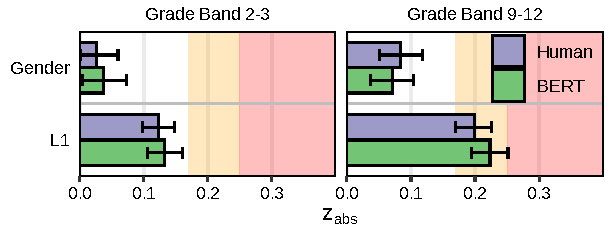
\includegraphics[width=8.2cm]{figures/20230504_ETS-DIF_BERT_zabs_ovr_edit.pdf}
    \caption{Estimates of overall DIF. Error bars indicate 95\% confidence intervals. Yellow shaded regions correspond to moderate DIF, and red shaded regions correspond to strong DIF.}
    \label{fig:zabs_ovr}
\end{figure}

\noindent \textbf{Human vs. BERT overall DIF} \;
Overall DIF of automated scores was highly similar to human scores. As seen in Figure \ref{fig:zabs_ovr}, green bars (representing BERT scores) are nearly commensurate with gray bars (representing human scores), with mostly overlapping 95\% confidence intervals. Yet, there was significantly more DIF in BERT scores compared to human scores with respect to L1 in Grade Band 9–12 ($\Delta z_{abs} = .025, CI_{95\%} = [.011, .039], p = 3.3 \cdot 10^{-4}$). In practical terms, however, an effect size of 0.025 standard deviations is very small. 

\noindent \textbf{Human vs. BERT individual item DIF} \;
In addition to overall DIF, we examined DIF of each individual item. Figure \ref{fig:zabs_itm} presents DIF of human and automated scores, for gender and L1, across Items 1–3, for each grade band. Human and automated scores are again quite consistent. For Grade Band 9–12, L1 DIF tends to be higher across all items; however, only Item 3 reaches statistical significance ($\Delta z_{abs} = .032, CI_{95\%} = [.010, .055], p = 3.3 \cdot 10^{-3}$). An effect size of 0.032 is very small.

\begin{figure}[h]
    \centering
    \hspace{-.6cm}
    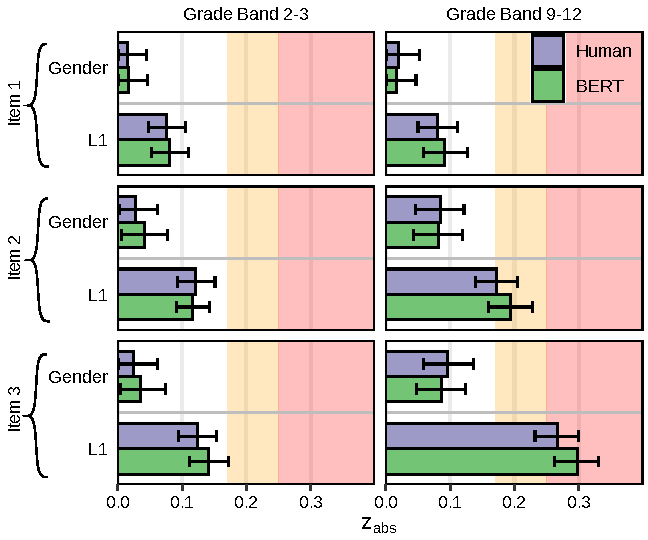
\includegraphics[width=8.2cm]{figures/20230504_ETS-DIF_BERT_zabs_itm_edit.pdf}
    \caption{Estimates of DIF for each of the 3 speaking items. Error bars indicate 95\% confidence intervals. Yellow shaded regions correspond to moderate DIF, and red shaded regions correspond to strong DIF.}
    \label{fig:zabs_itm}
\end{figure}

% % For adding bigger figures (across both columns)
% \begin{figure*}[htbp]
%     \centering
%     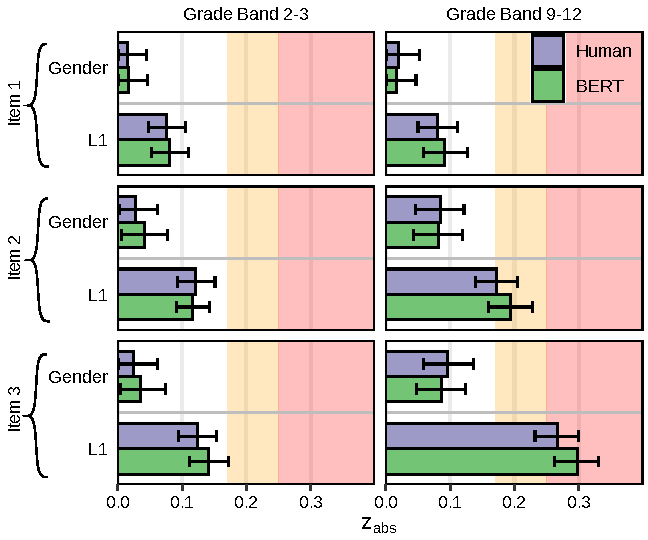
\includegraphics[width=16cm]{figures/20230504_ETS-DIF_BERT_zabs_itm_edit.pdf}
%     \caption{Estimates of DIF by gender and L1 for each of the 3 speaking items in grade-bands 2–3 and 9–12. Error bars indicate 95\% confidence intervals. Yellow shaded regions correspond to moderate DIF ($.17 < z_{abs} < .25$), and red shaded regions correspond to strong DIF ($z_{abs} > .25$).}
%     \label{fig:test}
% \end{figure*}

\subsection{DIF increases with item length}

Longer speaking items tended to exhibit more DIF than shorter speaking items. Automated scores, however, do not exacerbate this trend. 

In terms of item length, Item 3 was longer than Item 2, which was in turn longer than Item 1. Figure \ref{fig:zabs_itm} shows that DIF, too, generally increased in magnitude across items 1–3. Table \ref{itm_diff} presents the specific values of $\Delta z_{abs,ij}$ for all three item comparisons (corresponding to combinations of Item $i \neq j$) for each grade-band. 

\begin{table*}[ht]
\centering
\small  % comment out this line if wanted bigger font size
\begin{tabular}{lccccccc}
\toprule
    & \multicolumn{3}{c}{\textbf{Grade Band 2-3}} & \multicolumn{1}{c}{ } & \multicolumn{3}{c}{\textbf{Grade Band 9-12}} \\
    \cline{2-4}
    \cline{6-8}
    \textbf{Factor} & \textbf{2 - 1} & \textbf{3 - 1} & \textbf{3 - 2} & & \textbf{2 - 1} & \textbf{3 - 1} & \textbf{3 - 2} \\
    \midrule
    \multirow{2}*{Gender} & .012 & .010 & -.002 & & .065 * & .078 * & .013 \\
    & [-.030, .051] & [-.029, .049] & [-.042, .039] & & [.021, .110] & [.031, .116] & [-.032, .055] \\
    \multirow{2}*{L1} & .046 * & .053 * & .006 & & .087 * & .184 * & .097 * \\
    & [.009, .085] & [.010, .093] & [-.035, .046] & & [.043, .130] & [.139, .226] & [.056, .138] \\
    \bottomrule
    \end{tabular}
\caption{\label{itm_diff}
Differences in DIF between longer and shorter items, within each grade band, based on human ratings. "*" indicates that an estimate is statistically significant using B-H adjusted p-values. 95\% confidence intervals are presented in square brackets.}
\end{table*}

Although longer items tend to have more DIF, this general trend was not uniformly consistent across factors and grade-bands. Specifically, the trend was less consistent for gender: There were no statistically significant differences in Grade Band 2–3; and in Grade Band 9–12, Item 3 did not have more DIF than Item 2 at a statistically significant level. Additionally, for Grade Band 2–3, Item 3 did not have significantly more DIF than Item 2.

In order to determine if item-item differences were exacerbated by automated scoring, we computed second-order differences, $\Delta \Delta z_{abs}$. None of these values, however, were statistically significant. We conclude that the pattern of longer-items producing more DIF is consistent for both human and automated raters. 

\subsection{DIF is higher for older examinees}

In general, there is more DIF for older examinees (in Grade Band 9–12) compared to younger examinees (in Grade Band 2–3). Automated scores, however, do not exacerbate this trend.

There is significantly more DIF for Grade Band 9–12 compared to 2–3, in terms of both gender and L1. This trend can be seen clearly in Figure \ref{fig:zabs_itm}. Based on bootstrapped estimates for gender, $\Delta z_{abs} = .059$ ($CI_{95\%} = [.011, .100], p = 4.9 \cdot 10^{-3}$); and for L1, $\Delta z_{abs} = 0.082$ ($CI_{95\%} = [0.047, 0.120], p = 3.8 \cdot 10^{-6}$). 

When we examine individual items, this trend is present for items that are medium–long (Items 2 and 3) but not for short items (Item 1). Visually, this can be seen in Figure \ref{fig:zabs_itm}. Numerically, this is presented for human ratings in Table \ref{gr_diff}. 


\begin{table}[htbp]
\centering
\small  % comment out this line if wanted bigger font size
\begin{tabular}{p{0.8cm}ccc}
\toprule
\textbf{Factor} & \textbf{Item 1} & \textbf{Item 2} & \textbf{Item 3} \\
\midrule
\multirow{2}*{Gender} & .005 & .058 * & .072 * \\
            & [-.033, .042] & [.011, .105] & [.019, .118]\\
\multirow{2}*{L1} & .013   & .054 *  & .145 *  \\
 & [-.029, .057] & [.012, .098] & [.098, .193] \\
\bottomrule
\end{tabular}
\caption{\label{gr_diff}
Differences in DIF between grade-bands, based on human ratings, for each of the three speaking items. "*" indicates that an estimate is statistically significant using B-H adjusted p-values. 95\% confidence intervals are provided in square brackets.}
\end{table}

In order to determine if differences between grade-bands were exacerbated by automated scoring, we computed second-order differences, $\Delta \Delta z_{abs}$. None of these values, however, were statistically significant. We conclude that the trend of greater DIF in older examinees is consistent for both human and automated raters. 

\subsection{Severity of DIF depends on L1 and grade-band}

The magnitude and quantity of DIF varied by L1 background, and patterns were generally not consistent across grade-bands. Figure \ref{fig:z_ovr} depicts the magnitude and direction of DIF for gender and all L1 groups. For Grade Band 2–3, native speakers of Marshallese and Mayan languages showed evidence of moderate–strong DIF for human and BERT scores. DIF was negative for both L1 groups, indicating that these examinees fared worse on speaking items than their (equally-proficient) Spanish-speaking counterparts. 

\begin{figure*}[t]
    \centering
    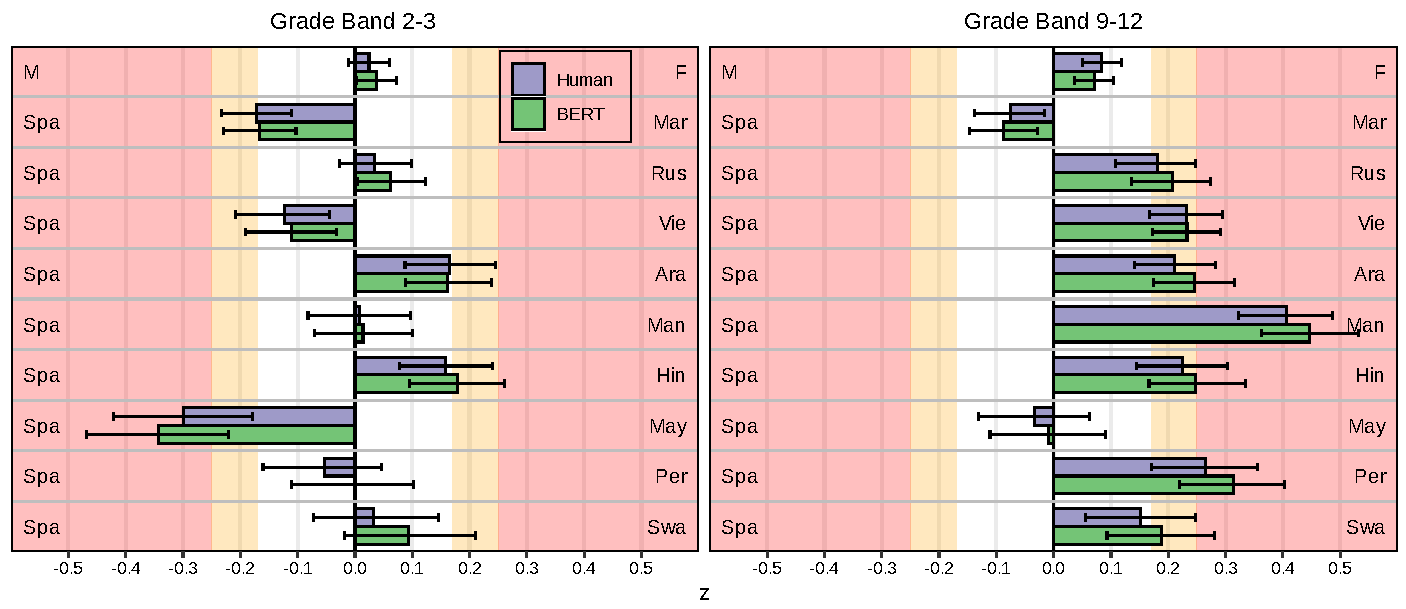
\includegraphics[width=16cm]{figures/20230504_ETS-DIF_BERT_z_ovr_edit.pdf}
    \caption{Estimates of direction and magnitude of overall DIF. Error bars indicate 95\% confidence intervals. Yellow shaded regions correspond to moderate DIF, and red shaded regions correspond to strong DIF. Reference groups are listed on the left of each chart (M = Male, Spa = Spanish); focal groups are listed on the right (L1 groups are abbreviated by the first three letters). DIF in the positive direction indicates that the focal group is favored.}
    \label{fig:z_ovr}
\end{figure*}

In Grade Band 9–12, examinees of nearly all L1 backgrounds fared better than native Spanish speakers. In this case, speaking items tended to disadvantage members of the reference group (i.e. examinees with Spanish L1 backgrounds). 

As with preceding analyses, DIF based on BERT scores aligned closely with DIF based on human scores. Although results showed that BERT exacerbated DIF in L1 as a whole (Section \ref{res_rq1}), analyses of individual L1 groups did not reveal any statistically significant differences between human and BERT scores. We also did not find any statistically significant differences between human and BERT scores when examining DIF at the individual item level (Appendix \ref{sec:appendix_z_itm}). 

\chapter{Discussion}

\subsection{Main findings}

Analysis of differential item functioning (DIF) revealed specific patterns of biases in human and automated scores of English speaking assessment. With respect to human scores, we found that there was more DIF for older examinees and for longer items. Based on commonly accepted standards regarding effect size, there was a moderate amount of overall DIF in Grade Band 9–12 based on examinees’ native language (L1) backgrounds. Automated scores generated by off-the-shelf BERT models closely matched human scores, yet BERT was found to exacerbate overall DIF for Grade Band 9–12 based on examinees’ native language (L1). The degree to which BERT exacerbated this bias, however, was very small.

\subsection{Causes of DIF}

Although our findings do not confirm any causes of DIF, they do allow us to rule out several possibilities. 

\noindent \textbf{Implicit bias} \;
Our automated scoring system was based exclusively on transcripts of examinees’ speech. No phonic information was used in the automated scoring process. It is notable, then, that there was no mitigation of DIF in automated scores using a text-based BERT model. In other words, removal of acoustic input did not reduce bias. From this, we conclude that examinees with \emph{identical} (transcribed) responses could not have received higher or lower scores, on average, based on gender or L1. 

Although text-based automated scores did not mitigate bias, this does not necessarily imply that human raters were unaffected by implicit bias. It is possible, for instance, that examinees with different accents also had different (transcribed) responses, which still affected human raters' judgment. 

\noindent \textbf{Transcription (in)accuracy} \;
Prior research shows that there are discrepancies in word error rate (WER) of automated transcription based on L1 (Anonymous). Specifically, automated transcription struggles with speakers of Vietnamese L1 backgrounds. Yet given the close correspondence between human and automated scores—for all examinees, not just Vietnamese examinees—it appears unlikely that transcription inaccuracies engender lower or higher scores. 

\subsection{Accuracy and DIF}

As the performance of automated scoring improves to match (or exceed) that of human raters, one might expect the magnitude of DIF to also match (or potentially reduce) that of human raters. For longer speaking items, however, we found that automated scores exceeded the performance of human raters, yet increased DIF. More research is needed to determine the relationship between performance of automated scoring systems and DIF.

\subsection{Limitations}

Our analyses are based around one metric of uniform DIF, $z$. The benefits of $z$ are that it is commonly used in practice, it is highly interpretable with well-established effect sizes, and it is easy to aggregate across items and focal groups. One of the drawbacks, however, is that it does not capture non-uniform DIF, and it is not ideal in terms of statistical power \citep{woods2013}. 

Consistent with other analyses of DIF, our study struggles to identify sources of DIF \citep{zumbo2007}. Although it is outside the scope of this study, a fine-grained analysis of examinees’ language, especially based on L1, could provide insight. Additionally, it could be beneficial to explore the possibility of modifying BERT using debiasing techniques \citep{sun2019mitigating}. Not only could these techniques potentially reveal sources of DIF, but they may be able to reduce DIF of human raters.

\chapter{Appendices}

\section{L1 Groups}
\label{sec:appendix_lang}

In selecting L1 groups, one of our aims was to represent languages from around the globe. In some cases, this required grouping languages to reach an adequate sample size for statistical analyses. Given the constraints of sample size, we tried to ensure that L1 groups were as geo-historically related to each other as possible \citep{brown2005encyclopedia}. The four composite L1 groups in our study were (1) Hindi, (2) Mayan languages, (3) Persian, and (4) Swahili. For simplicity, we refer to composite L1 groups by the predominate language within each group, with the exception of Hindi (in order to remain consistent with a prior study). It would be more accurate, however, to refer to the L1 groups as (1) Indo-Aryan, (2) Indigenous languages of Central and South America, (3) Indo-European languages of the Middle East, and (4) Niger-Congo languages. 

The languages within each of the composite L1 groups are presented in Table \ref{lang_grp}. Note that the names of languages are derived from states’ departments of education, which do not follow the same naming conventions. We made minor changes in compiling the list of languages (e.g. changing “Panjabi” to “Punjabi”). 

\begin{table*}[htbp]
\centering
% \small  % comment out this line if wanted bigger font size
\begin{tabular}{lccccccc}
\toprule
    & \multicolumn{2}{c}{\textbf{Grade Band 2-3}} & \multicolumn{1}{c}{ } & \multicolumn{2}{c}{\textbf{Grade Band 9-12}} \\
    \cline{2-3}
    \cline{5-6}
     \textbf{Language} & \textbf{n} & \textbf{\%} & & \textbf{n} & \textbf{\%} \\
    \midrule
\textbf{Hindi} & & & & & \\
\hspace{3mm} Punjabi & 157 & 37.7 & & 75 & 40.5 \\
\hspace{3mm} Hindi & 124 & 29.8 & & 39 & 21.1 \\
\hspace{3mm} Urdu & 65 & 15.6 & & 35 & 18.9 \\
\hspace{3mm} Gujarati & 46 & 11.1 & & 30 & 16.2 \\
\hspace{3mm} Marathi & 24 & 5.8 & & 6 & 3.2 \\
\textbf{Mayan languages} & & & & & \\
\hspace{3mm} Mayan languages & 212 & 89.1 & & 214 & 82.9 \\
\hspace{3mm} Q'anjob'al & 24 & 10.1 & & 40 & 15.5 \\
\hspace{3mm} Quechua & 1 & 0.4 & & 3 & 1.2 \\
\hspace{3mm} Q'eqchi & 1 & 0.4 & & 1 & 0.4 \\
\textbf{Persian} & & & & & \\
\hspace{3mm} Persian & 209 & 70.8 & & 97 & 49.2 \\
\hspace{3mm} Kurdish & 76 & 25.8 & & 87 & 44.2 \\
\hspace{3mm} Farsi & 10 & 3.4 & & 13 & 6.6 \\
\textbf{Swahili} & & & & & \\
\hspace{3mm} Swahili & 89 & 42.6 & & 120 & 55.3 \\
\hspace{3mm} Nuer & 37 & 17.7 & & 28 & 12.9 \\
\hspace{3mm} Niger-Kordofanian languages & 16 & 7.7 & & 16 & 7.4 \\
\hspace{3mm} Dinka & 19 & 9.1 & & 11 & 5.1 \\
\hspace{3mm} Kinyarwanda & 7 & 3.3 & & 19 & 8.8 \\
\hspace{3mm} Wolof & 15 & 7.2 & & 10 & 4.6 \\
\hspace{3mm} Fulah & 10 & 4.8 & & 5 & 2.3 \\
\hspace{3mm} Igbo & 7 & 3.3 & & 5 & 2.3 \\
\hspace{3mm} Yoruba & 3 & 1.4 & & 1 & 0.5 \\
\hspace{3mm} Hausa & 1 & 0.5 & & 1 & 0.5 \\
\hspace{3mm} Akan & 2 & 1 & & 0 & 0 \\
\hspace{3mm} Shona & 2 & 1 & & 0 & 0 \\
\hspace{3mm} Chichewa; Chewa; Nyanja & 0 & 0 & & 1 & 0.5 \\
\hspace{3mm} Kirundi & 1 & 0.5 & & 0 & 0 \\
    \bottomrule
    \end{tabular}
\caption{\label{lang_grp}
Languages of composite L1 groups by grade-band.}
\end{table*}

There is a great deal of heterogeneity within L1 groups, as with gender, and as with all other demographic characteristics. We note that L1 is not synonymous with cultural identity, racial identity, geographic identity, or preferred language. Despite these limitation, in the context of English speech assessment, we believe L1 is a more relevant construct than, say, conventional racial categories (e.g. White, Asian, Black). 

\section{BERT Performance Metrics}
\label{sec:appendix_perf}

Performance metrics of all six BERT models are presented in Table \ref{bert_perf}. Approximately 10\% of all responses were scored by two human raters, independently, which provides the basis for comparisons between human and BERT performance. 

\begin{table*}[ht]
\centering
\small  % comment out this line if wanted bigger font size
\begin{tabular}{lccccccccccccc}
\toprule
    & \multicolumn{6}{c}{\textbf{Grade Band 2-3}} & \multicolumn{1}{c}{ } & \multicolumn{6}{c}{\textbf{Grade Band 9-12}} \\
    \cline{2-7}
    \cline{9-14}
    & \multicolumn{2}{c}{\textbf{Acc.}} & \multicolumn{2}{c}{\textbf{r}} & \multicolumn{2}{c}{\textbf{QWK}} & \multicolumn{1}{c}{ } & \multicolumn{2}{c}{\textbf{Acc.}} & \multicolumn{2}{c}{\textbf{r}} & \multicolumn{2}{c}{\textbf{QWK}} \\
    \textbf{Item} & \textbf{Human} & \textbf{BERT} & \textbf{Human} & \textbf{BERT} & \textbf{Human} & \textbf{BERT} & & \textbf{Human} & \textbf{BERT} & \textbf{Human} & \textbf{BERT} & \textbf{Human} & \textbf{BERT} \\
    \midrule
    1 & .911 & .896 & .793 & .713 & .792 & .713 & & .929 & .904 & .920 & .895 & .920 & .895 \\
    2 & .756 & .685 & .898 & .861 & .898 & .859 & & .728 & .700 & .911 & .910 & .911 & .909 \\
    3 & .614 & .618 & .834 & .834 & .834 & .829 & & .694 & .707 & .841 & .885 & .609 & .884 \\
    \bottomrule
    \end{tabular}
\caption{\label{bert_perf}
 “human” refers to human-human comparisons. The number of observations that were scored by two human raters ranges from 1,567–1641 for Grade Band 2–3, and from 1,254–1,293 for Grade Band 9–12. “BERT” refers to human-BERT comparisons. The number of observations in the testing sets were 4,185 for Grade Band 2–3, and 3,306 for Grade Band 9–12.}
\end{table*}

\section{Human vs. BERT DIF for each item}
\label{sec:appendix_z_itm}

Figure \ref{fig:z_itm} presents the magnitude and direction of DIF of Items 1-3 for grade-bands 2-3 and 9-12, based on gender and all nine L1 focal groups separately.

\begin{figure*}[t]
    \centering
    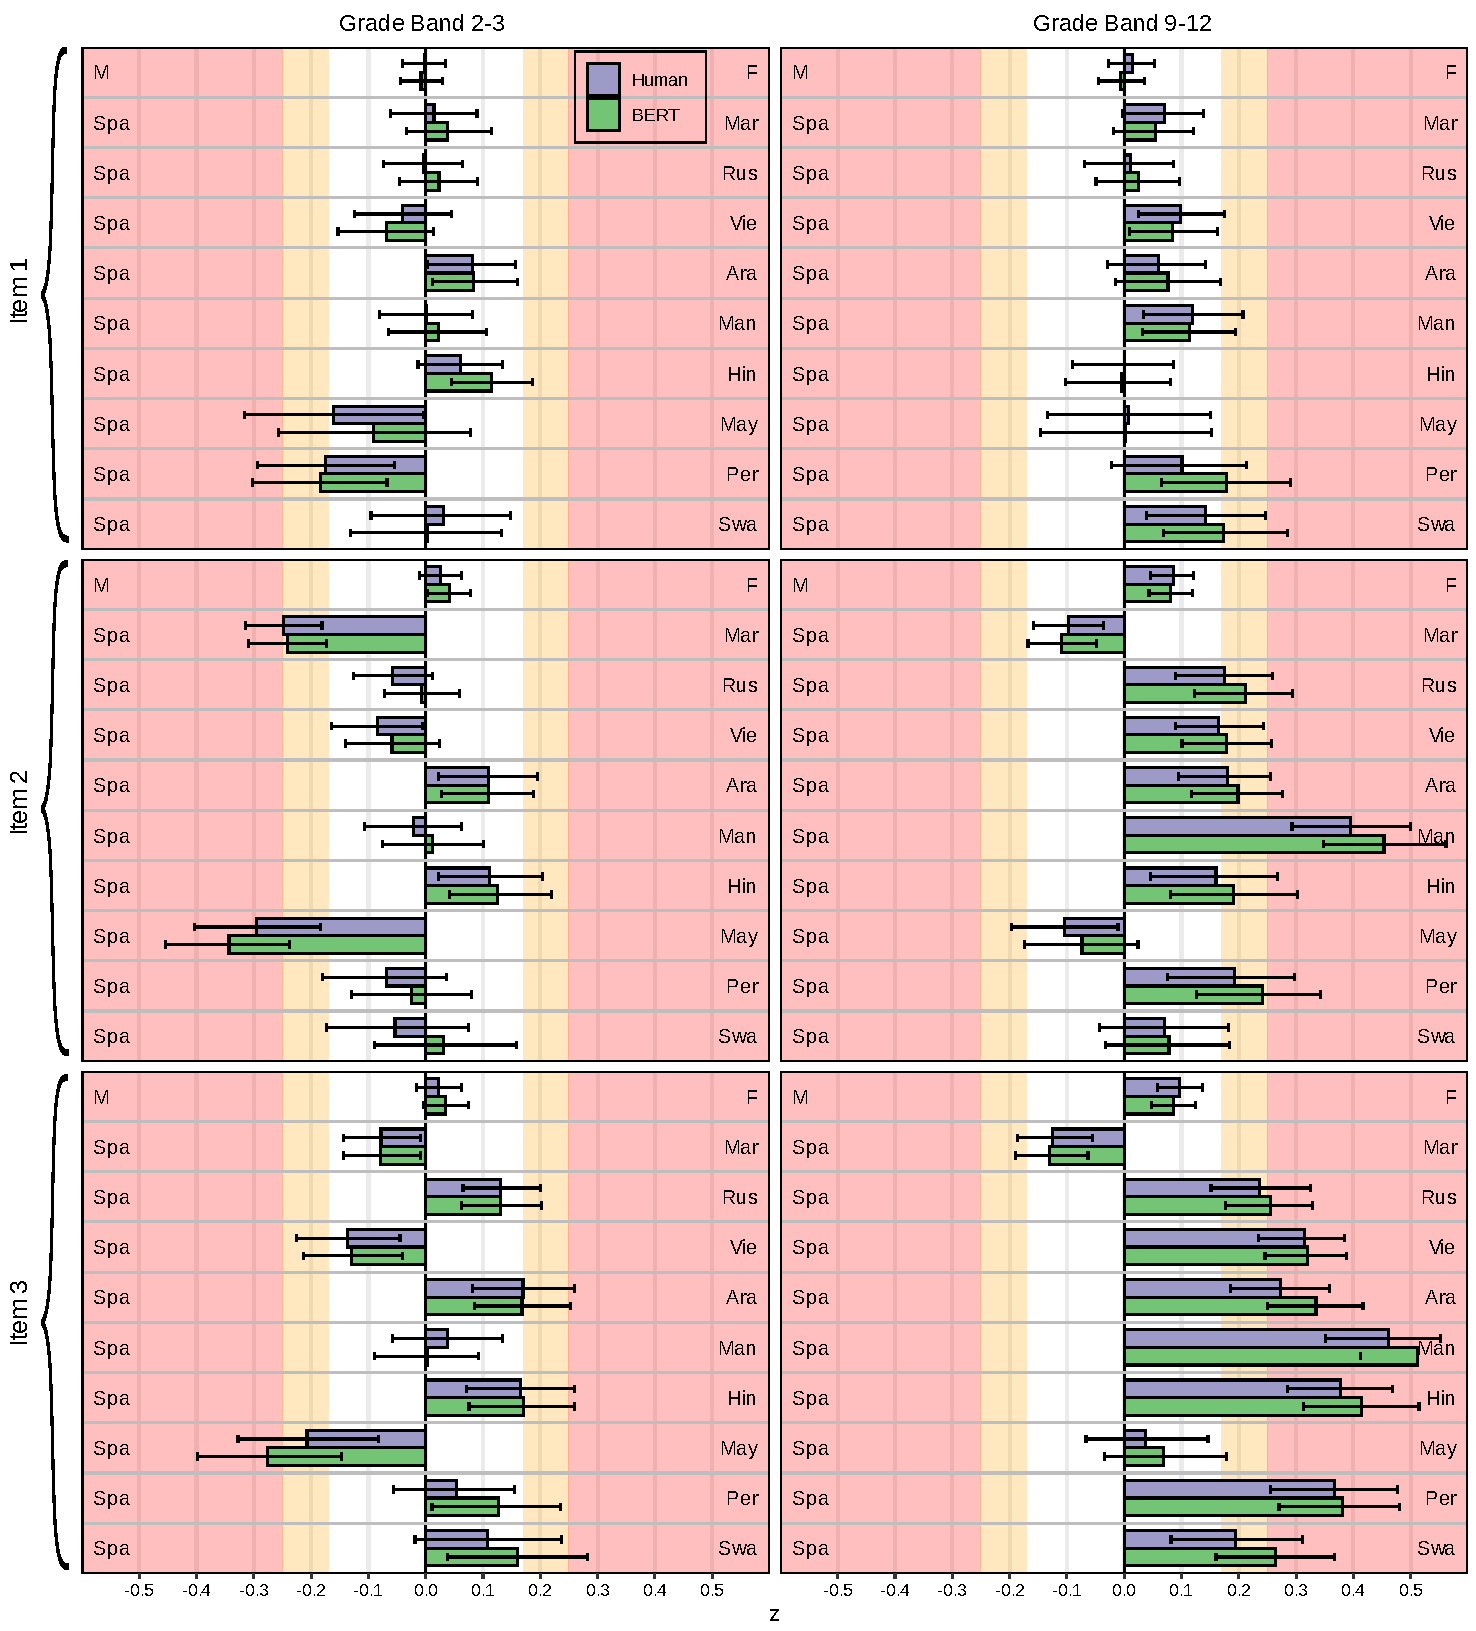
\includegraphics[width=16cm]{figures/20230504_ETS-DIF_BERT_z_itm_edit.pdf}
    \caption{Estimates of direction and magnitude of DIF for each of the three speaking items. Error bars indicate 95\% confidence intervals. Yellow shaded regions correspond to moderate DIF, and red shaded regions correspond to strong DIF. Reference groups are listed on the left of each chart (M = Male, Spa = Spanish); focal groups are listed on the right (L1 groups are abbreviated by the first three letters). DIF in the positive direction indicates that the focal group is favored.}
    \label{fig:z_itm}
\end{figure*}

%\bibliography {bib/network,bib/naming}    % bibliography references
\bibliography{20230507_dissertation}
%\bibliographystyle {thesis}
%\bibliographystyle{apa-like}
%\bibliographystyle {uclathes}
%\bibliographystyle{apalike}
%\bibliographystyle{acl_natbib}
\bibliographystyle{plainnat}

\end {document}

